\section{区块链辅助保障：选择与明确的实现模式}
\subsection{使用账本的决策}\label{sec:ledger-choice}

账本采用决策从写入者、状态和权限出发。W\"ust 和 Gervais 围绕是否需要存储共享状态、写入者数量及其信任关系，以及可信参与方的可用性组织决策\citep{wust2018need}。Locher 等考察可信第三方的哪些功能可以由分布式一致性替代\citep{locher2018when}。对于任务保障，相关要求是：任何单一组织都不能悄然改变已接受的成员资格、策略或撤销历史，同时授权参与方保留可相互验证的状态。

在联盟示例中，A 不能独自替换传感器接受策略，C 不能在网关事件发生后删除此前已确认的批次，D 也不能自行宣布其数据已获联盟接受。四个独立组织可以共同验证这些转换。许可账本是实现这一要求的一种方式。

最强的替代方案是一种透明服务，其检查点和状态转换由独立见证方按照相同授权规则检查。该服务可以满足相同的安全性要求。仅检查一致性的见证方能够发现或暴露不一致历史，但这一行为本身并不能证明策略变更已经获得授权。增加共同策略验证可以补足这一环节。因此，第~\ref{sec:trace} 节的回放发现，账本与策略验证日志产生等价决策。架构选择随后取决于实现复杂度、隐私、可用性、恢复和实测成本。图~\ref{fig:blockchain-boundary} 汇总这种共享状态服务选择。

治理可行性同样是采用条件。TradeLens 虽然在技术上可行，但未能实现所需的全球行业协作和商业可行性，Maersk 与 IBM 因而终止了该平台\citep{maersk2022tradelens}。这一海事案例说明需要评估激励、参与、退出和运行责任。

\begin{figure}[!htbp]\centering
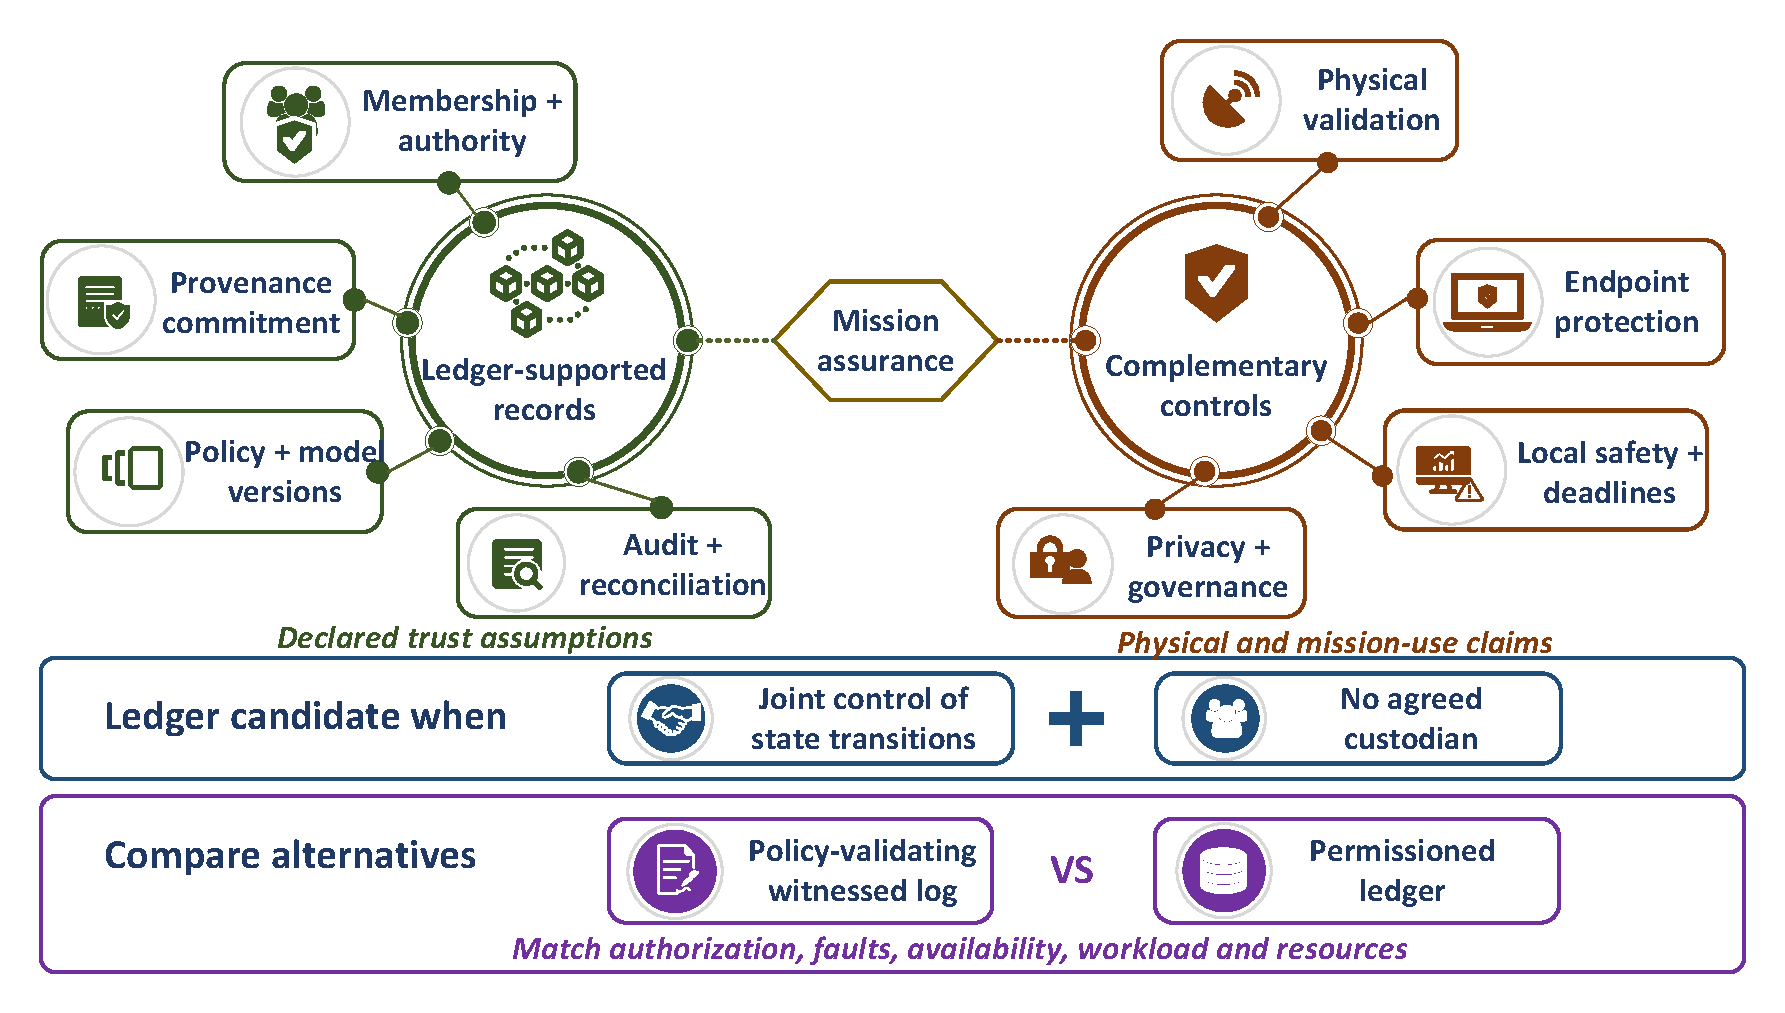
\includegraphics[width=\textwidth]{figures/figure-06-blockchain-boundary.pdf}
\caption{基于需求的共享状态服务选择。在匹配的治理保障条件下，比较具有策略验证能力的见证日志与许可账本。物理评估与本地安全仍由应用负责。}\label{fig:blockchain-boundary}
\end{figure}

\subsection{任务要求与候选共识机制}\label{sec:consensus}

如 \v{S}varcmajer 等所倡导\citep{svarcmajer2026consensus}，基于需求的选择流程在选择协议前先明确故障模型。此处联盟设计假定：四个独立控制的岸端节点中，至多存在一个拜占庭管理域。在 USV 分区期间必须保持安全性；当无法获得有响应的法定人数时，新的全局决策可以停止。示例协调截止时间为事件可供岸端处理后的 60 s。一次任务期间成员保持稳定，并通过共同批准的纪元转换来变更。岸端节点具有足够的计算和供电能力；UUV 不参与共识。共识流量使用岸端/无线电基础设施，只有紧凑的证据承诺经过声学链路。

表~\ref{tab:consensus} 比较代表性协议类别。正常路径消息复杂度是一项选择指标，其含义取决于批处理、签名聚合、传播和视图变更。容错能力与活性假设仍具有决定作用。尤其是，采用有向无环图（DAG）组织数据，并不能免除明确说明由何种一致性协议对数据排序或认证的要求。

Raft 和拜占庭协议解决不同的故障问题\citep{raft2014,pbft1999,hotstuff2019}。CometBFT 使用自身基于轮次的共识和 gossip 传播规则\citep{cometbft2026}；Narwhal 是传播/内存池组件，Tusk 则提供关联的排序协议\citep{narwhal2022}。BUS 所实现的基于权威节点的 UAV 采集，展示了将功能部署在能力充足的验证节点上的做法\citep{islam2019bus}。轻量级 IoT 方案同样支持将共识移出受限端点\citep{dorri2017towards}；评估这种优化时，需要同时考虑由此形成的管理依赖。

\begin{table}[H]\footnotesize
\caption{候选共识机制与任务要求的比较。消息复杂度阶数描述代表性的正常路径；恢复成本可能更高。}\label{tab:consensus}
\begin{tabularx}{\textwidth}{@{}P{25mm}YYY@{}}\toprule
\textbf{类别} & \textbf{故障模型与分区行为} & \textbf{时延、流量及资源影响} & \textbf{适用场景}\\\midrule
Raft & 崩溃故障；推进需要多数节点 & 领导者复制，每条记录通常为 $O(n)$ 次交换；服务器成本低；受管理的成员变更 & 单一责任运营方及仅考虑崩溃的副本；不足以应对拜占庭联盟管理方\\
经典 BFT / SmartBFT & 拜占庭故障；通常要求 $n\geq3f+1$ 和 $2f+1$ 个有响应的投票 & 多阶段通信，通常为 $O(n^2)$；超时/视图变更成本；能力充分且稳定的节点 & 小型独立岸端联盟；本文选择的 Fabric 排序候选\\
HotStuff & 拜占庭故障；法定人数及部分同步条件下的活性 & 法定人数证书和流水线带来线性正常路径通信；密码聚合与领导者可用性重要 & 经实测证明负载收益的较大型高能力联盟\\
CometBFT & 拜占庭故障；超过三分之二投票权；轮次/锁定规则 & Tendermint 风格的提议/投票与 gossip；延迟下会发生超时；传播成本取决于实现 & 应用特定的复制状态机；不能仅因同属 BFT 就归为 HotStuff\\
基于权威节点 & 具名验证者；韧性取决于具体协议 & 挖矿成本低；必须明确调度/最终性及法定人数假设 & 只有具体权威协议满足故障要求时，才适用于受控联盟\\
基于 DAG（Narwhal/Tusk） & 可靠数据传播加明确的 BFT 排序协议 & 并行传播与存储；仍需考虑异步推进假设与通信成本 & 有资源证据支持的高吞吐岸端服务；不能绕过声学分区问题\\
面向 IoT 的设计 & 常采用簇头、可信管理者或受限验证者集合 & 将端点工作转移到高能力节点；信任与可用性假设随之变化 & 网关介导的数据采集；仅当其委托信任符合任务需求时选择\\\bottomrule
\end{tabularx}\end{table}

基础设施与应用的故障假设分别陈述。拜占庭排序服务关注副本任意行为下的一致性，并不能阻止获授权生产者提供虚假观测。背书限制谁可以批准拟议状态更新，链码则定义被批准的确定性规则。合约可能一致地执行一条不适当的规则，因此策略批准还需要有关任务后果的证据。应用必须明确紧急权限能否绕过通常的背书，以及如何记录和审查该例外。没有明确例外时，必需签名方不可用就意味着有意停止授予新的全局权限。

分区容忍性也有两层必须区分的含义。安全性是在消息延迟或不可用时，保留一致的已接受历史。可用性关注特定请求能否在截止时间前取得所需排序和应用批准。USV 断连时，岸端法定人数仍可能正常工作，从而允许岸端撤销继续推进，而 UUV 依据缓存权限运行。若岸端法定人数本身被分割，即使网关恢复连接，新的全局更新仍可能停止。评估应独立改变这两种分区位置。经典的一致性/可用性结果为网络分区下的这一区分提供动机\citep{gilbert2002brewer}；它们并不规定航行器的本地安全策略。

由此得到三种场景决策。单机构检查任务可以采用经过认证的数据库或见证日志，并增加 Raft 复制以获得崩溃故障下的可用性。四组织响应任务需要拜占庭排序加共同应用授权，或者等价的验证日志；当前 Fabric SmartBFT 是一个具体候选\citep{fabric2026bft}。断连的 UUV 群体使用签名本地记录、存储转发传输和有界委托，不要求声学共识。增加验证者数量，只有在增加独立故障域且保持法定人数可达时才有帮助。实际时延和能耗必须针对所选部署测量。

\subsection{联盟溯源与撤销模式}\label{sec:pattern}

该明确模式将证据承诺与分区后协调相结合；表~\ref{tab:blockchain-patterns} 将其与成员资格、版本协调和审计联系起来。

\begin{table}[H]\small
\caption{账本角色及其对应的应用要求。}\label{tab:blockchain-patterns}
\begin{tabularx}{\textwidth}{@{}P{24mm}YY@{}}\toprule
\textbf{角色} & \textbf{共享状态} & \textbf{所需互补证据}\\\midrule
成员资格 & 角色、委托、密钥纪元 & 身份证明与受保护的密钥保管\\
承诺 & 批次根、序列号、保留对象引用 & 签名源记录和可检索的载荷\\
版本协调 & 策略/模型哈希和批准纪元 & 模型验证与部署证据\\
审计 & 决策、证据链接和生效时间历史 & 完整捕获与独立审查\\
协调 & 已收到批次、缺口、冲突和判断 & 受保护的时钟/计数器与离线权限历史\\\bottomrule
\end{tabularx}\end{table}

\textbf{部署与背书。}A--D 各组织在能力充分的岸端基础设施上，分别部署一个背书对等节点和一个独立排序节点。示例 BFT 服务包含四个排序节点，在其协议假设下容忍一个拜占庭节点。管理上的分离提供独立故障域。应用背书规则为 \texttt{AND(A, B, OR(C, D))}；通道配置和链码定义批准要求相同的联盟权限。A 和 B 是必需方，因此即使仍有三个排序节点响应，应用也可能停止推进。USV 负责转发和缓存签名证据，没有共识投票权。分区中的网关缓存批次，并在重连后进行幂等重试。UUV 安全控制始终遵循其本地运行边界。

\textbf{状态与编码。}状态键包括 mission/policy/epoch、producer/key/history、delegation/identifier、batch/producer/sequence 和 judgment/record/policy，分别表示任务/策略/纪元、生产者/密钥/历史、委托/标识符、批次/生产者/序列，以及判断/记录/策略。定长源记录体包含：各一字节的版本与类型、两个 16 字节的任务/生产者标识符、各四字节的序列与权限纪元字段、两个八字节的事件时间边界，以及三个分别对应策略、载荷、父项/根的 32 字节哈希。这些字段合计 154 字节。整数采用网络字节序；时间为相对于声明的任务纪元的有符号秒数。加上 64 字节 Ed25519 签名后，一条记录为 218 字节。域分离签名和哈希绑定记录类型与版本。批次采用相同的记录体布局，使用 Merkle 根和前一批次根，并增加两字节的记录数：签名前为 156 字节，签名后为 220 字节。十条签名记录保留在链下。网关的规范化 JSON 应用载荷为 525 字节。

\textbf{确定性的链码操作。}\texttt{CommitBatch} 读取任务纪元、网关角色和最新批次序列；验证紧凑网关签名与策略绑定；拒绝不一致序列或标识符相同而内容不同的重复项；并记录根。内容完全相同的重试返回已有结果。这提交的是可审计批次，并不声称每个叶记录都适合使用。\texttt{JudgeRecord} 验证提交的源签名和包含证明，读取生产者的历史密钥状态与委托，并依据第~\ref{sec:trace} 节的区间规则，写入独立的合格/已撤销/已隔离判断。\texttt{UpdatePolicy} 和 \texttt{RevokeKey} 要求联盟背书规则和单调递增纪元；撤销记录保留生效时间。决策读取的所有状态均进入 Fabric 读集，使验证能够拒绝基于过时状态的并发更新。链码执行期间不获取外部时钟或预言机值；这些输入由获授权提交的证据提供。

\textbf{提交状态与受限验证。}Fabric 的排序先于对等节点验证，因此区块包含关系并不能证明世界状态更新有效\citep{androulaki2018hyperledger,hyperledger2026fabric}。观察到有效提交后，满足 A+B+（C 或 D）的三个不同组织签署应用回执，内容包括任务、策略/权限纪元、批次根、序列、事件跨度和记录数。回执签署代码必须检查提交验证状态及预期应用状态。UUV 根据固定信任的纪元检查授权签名者身份、签名、单调递增的检查点序列、源记录签名和 Merkle 分支。十个叶节点补齐至 16 个时，分支包含四个 32 字节哈希。这些检查在固定信任的密钥下，建立共同证明的应用检查点与包含关系；它们不构成对全部 Fabric 共识和对等节点验证执行过程的原生验证。新纪元需要来自当前固定信任纪元的经过认证的转换。回执构成额外的应用信任边界，需要实现和测试。

\subsection{通信预算与分区敏感性}\label{sec:budget}

回执路径与检索路径满足不同的证据需求。收到检查点的航行器可以验证：独立组织在固定信任的权限纪元下确认了已提交的根。要评估观测，它仍需获取相关叶记录、包含路径，以及必要的数据源或转换证据。因此，只传递承诺的接触时段所支持的主张，比完整证据交付更窄。检索策略可以优先处理近期且后果重大的产品，把大批量图像推迟至更高带宽的接触时段，同时记录哪些必需输入仍不可用。检索失败表示证据缺失，不能表示完整性检查成功。

时钟与密钥转换也影响证明的可用期限。新策略发布后，缓存检查点仍是历史承诺的证据，但它能否支持新决策，取决于依赖策略和经过认证的转换历史。时钟不确定的航行器不能仅检查账本根，就认定到期条件仍然成立。它需要有界时间区间，或采用更严格的后备策略。同样，新的回执也无法使不可信的采集时间戳变得可信。这些要求将应用层证明与回放所使用的相同时间假设绑定，并明确受限验证方在这些假设失效时必须采取的行动。

Ed25519 签名长度为 64 字节\citep{rfc8032}；ML-DSA-44 签名长度为 2420 字节\citep{fips204}。预算比较这两种紧凑应用签名配置。Fabric 注册证书、背书、提案响应、读写集和信封，会增加取决于部署的字节量。只有网关在岸端网络上传输这些完整事务。完整事务大小和资源成本取决于配置的 Fabric 实现；525 字节的 JSON 数值仅覆盖网关的应用载荷。

对于大小为 $B$ 字节、净载荷速率为 $R$ bit/s 的消息，串行化传输时间下界为 $8B/R$。表~\ref{tab:budget} 使用 100、1000 和 5000 bit/s 作为场景输入。计算不包含传播、等待接触、调制解调器成帧、BPSec 开销、丢失、重试，以及证书/纪元更新。这些因素会增加端到端时延，必须针对明确的调制解调器与传输配置另行加入。

\begin{table}[H]\small
\caption{应用消息串行化传输时间下界。所有大小均由第~\ref{sec:pattern} 节的编码计算；ML-DSA 数值通过替换为标准化签名长度得到。}\label{tab:budget}
\begin{tabularx}{\textwidth}{@{}Yrrrr@{}}\toprule
\textbf{消息} & \textbf{字节} & \textbf{100 bit/s} & \textbf{1 kbit/s} & \textbf{5 kbit/s}\\\midrule
Ed25519 源记录 & 218 & 17.44 s & 1.744 s & 0.349 s\\
Ed25519 批次承诺（10 条记录） & 220 & 17.60 s & 1.760 s & 0.352 s\\
十条完整 Ed25519 记录 & 2180 & 174.40 s & 17.440 s & 3.488 s\\
ML-DSA-44 批次承诺 & 2576 & 206.08 s & 20.608 s & 4.122 s\\
Ed25519 记录+分支+共同回执 & 697 & 55.76 s & 5.576 s & 1.115 s\\\bottomrule
\end{tabularx}\end{table}

697 字节的下行内容包括：218 字节源记录、128 字节分支、两字节叶索引、156 字节检查点、一字节签名者位图，以及三个 64 字节签名。按每分钟一个十记录批次计算，220 字节承诺平均需要约 29.3 净 bit/s，而发送全部十条签名记录需要约 290.7 bit/s。因此，只传递承诺可以适应某些无法承载完整证据的接触时段，代价是需要后续检索，且即时评估不完整。以相同频率发送一个含十条记录的 ML-DSA-44 批次承诺，需要约 343.5 bit/s。假定公钥已预先配置；密钥分发与后量子验证时间属于另行计算的成本。

分区敏感性计算覆盖 63 种配置：验证者数为 4、7 和 10；响应数分别为法定人数减一、法定人数，以及全部验证者；分区持续时间为 0、10、30、58、59、60 和 120 s。假设恢复接触后的延迟分别为账本路径 2 s、验证日志路径 1 s，在法定人数可达时，60 s 截止时间分别容许最长 58 s 和 59 s 的分区。低于法定人数时，两者都不能完成新的共同决策。除排序法定人数外，还必须检查应用背书可用性。
